% Условная компиляция для самостоятельной работы
\ifdefined\mainfile
    % Если это часть основного файла, не добавляем начало и конец документа
\else
    \documentclass[12pt, a4paper]{report}
    \usepackage{/Users/vladbelousov/Desktop/Semestr_4-FP-NSU/Настройка/library}
    \usepackage[utf8]{inputenc} % Подключение поддержки UTF-8
    \begin{document}
\fi

%%-------------------------------%%

\chapter{Вариационное исчисление.}

\section{Примеры задач вариационного исчисления}

\textit{Задача математического анализа: } 



Есть кривая заданная функцией \( f(x) \) найти точки экстремума: 

\[  f'(x)=0 \Rightarrow {x_1,x_2}-{\text{точки, подозреваемые на экстремум}  }   \] 
\begin{gather*}
    f''(x_1)<0 \Rightarrow x_1  - \max  \\
    f''(x_2)>0 \Rightarrow x_2 - \min    
\end{gather*}

\textit{Задача вариационного исчисления:} 

Функционал: \( I [y]= \int_{x_0}^{x_1}F(x,y(x),y'(x))dx  \) 

Найти функцию \( y(x) \) такую, что \( I[y] \) принимает \( \min  \) или \( \max  \) 

\begin{flushleft}
    Пример 1 : задача наискорейшего спуска (задача Брахистохроне)
\end{flushleft}

Найти кривую \( y(x) \)  по которой тело из точки А в точку В попадет за наименьшее время. 

\begin{center}
    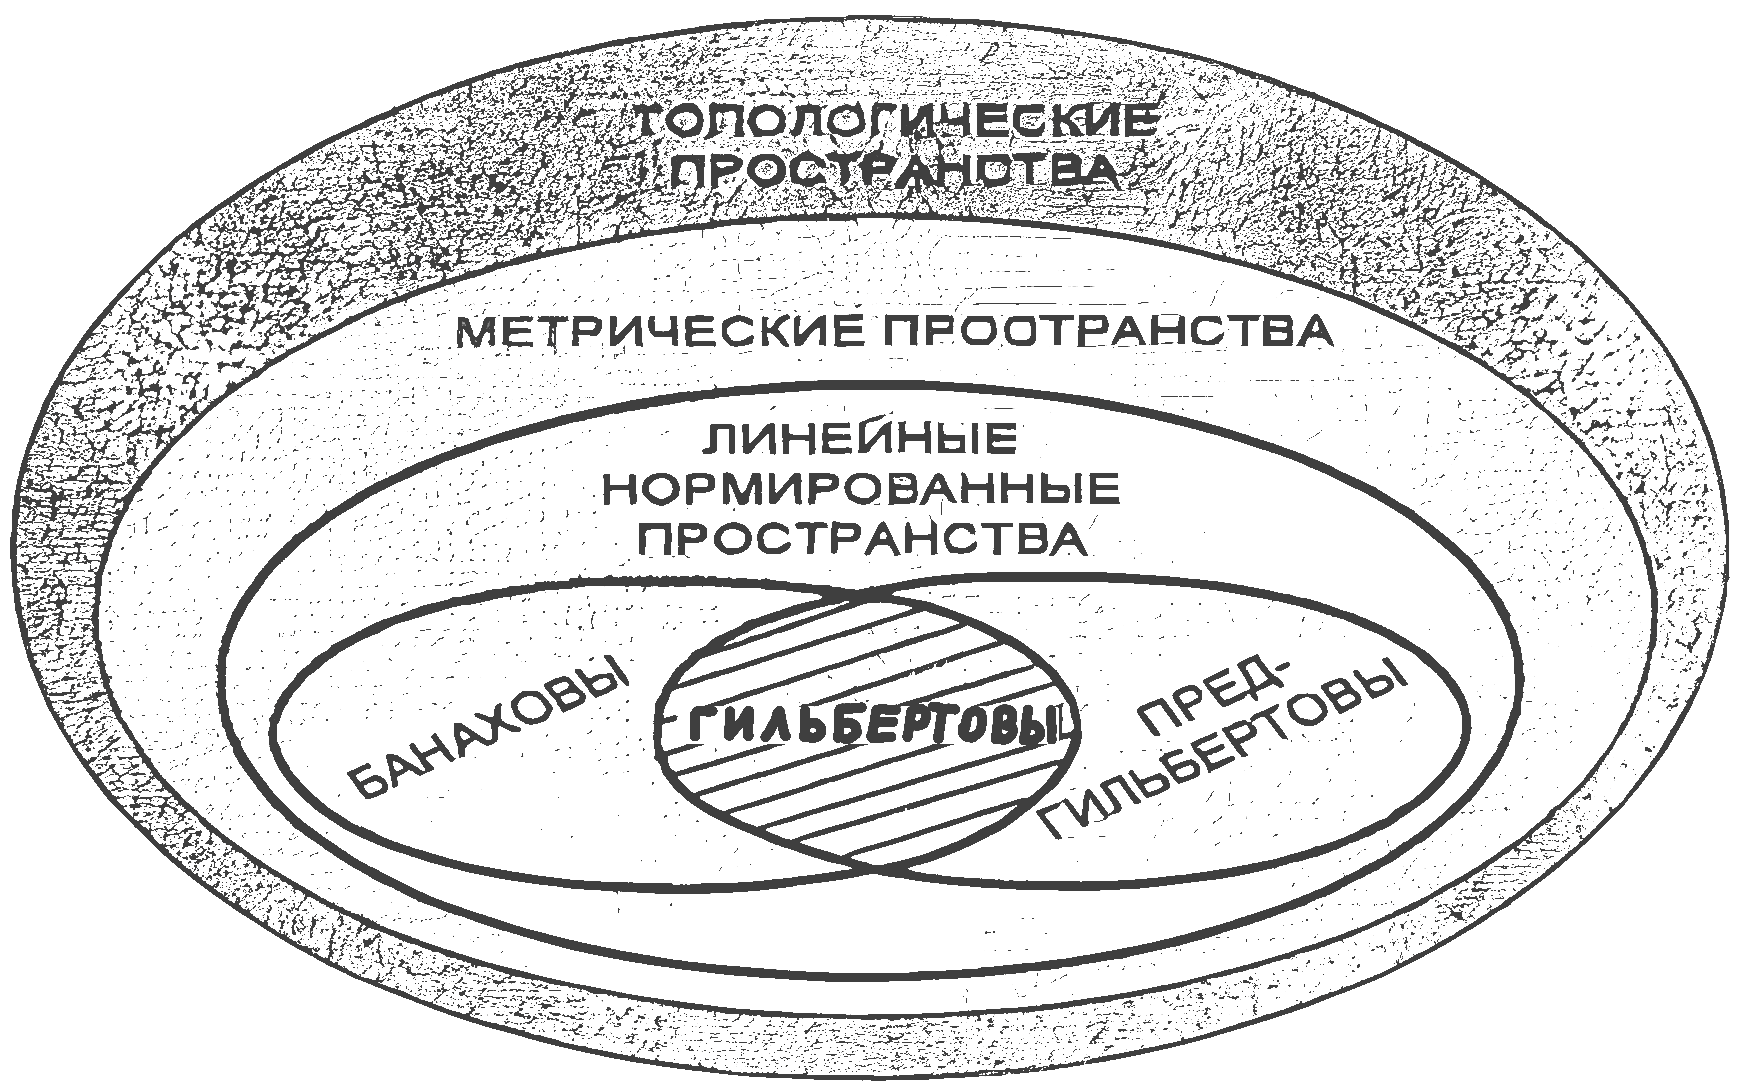
\includegraphics[width=0.5\textwidth]{/Users/vladbelousov/Desktop/Semestr_4-FP-NSU/ДфУ/Лекции_по_дням/image/1.png}
\end{center}

\begin{gather*}
   \text{З.С.Э: }  mgy_0+0= mgy(x)+ \frac{m |v| ^2}{2} \\
    \lvert v  \rvert =\sqrt{v_x ^2 + v_y ^2} = \sqrt{\left( \frac{\partial x}{\partial t}  \right) ^2 +\left( \frac{\partial y }{\partial t}  \right) ^2 }= \sqrt{1+(y'(x))^2} \frac{dx}{dt} \\
    \sqrt{2g(y_0- y(x)) }= |v|= \sqrt{1+(y(x)')^2} \frac{dx}{dt} \\
    T= \int_{0}^{T}dt= \int_{x_0 }^{x_1} \frac{\sqrt{1+(y'(x))^2}}{\sqrt{2g(y_0+ y(x)) }} dx   
\end{gather*}

\begin{flushleft}
    Пример 2 : задача поверхности вращения наименьшей площади. 
\end{flushleft}

\begin{center}
    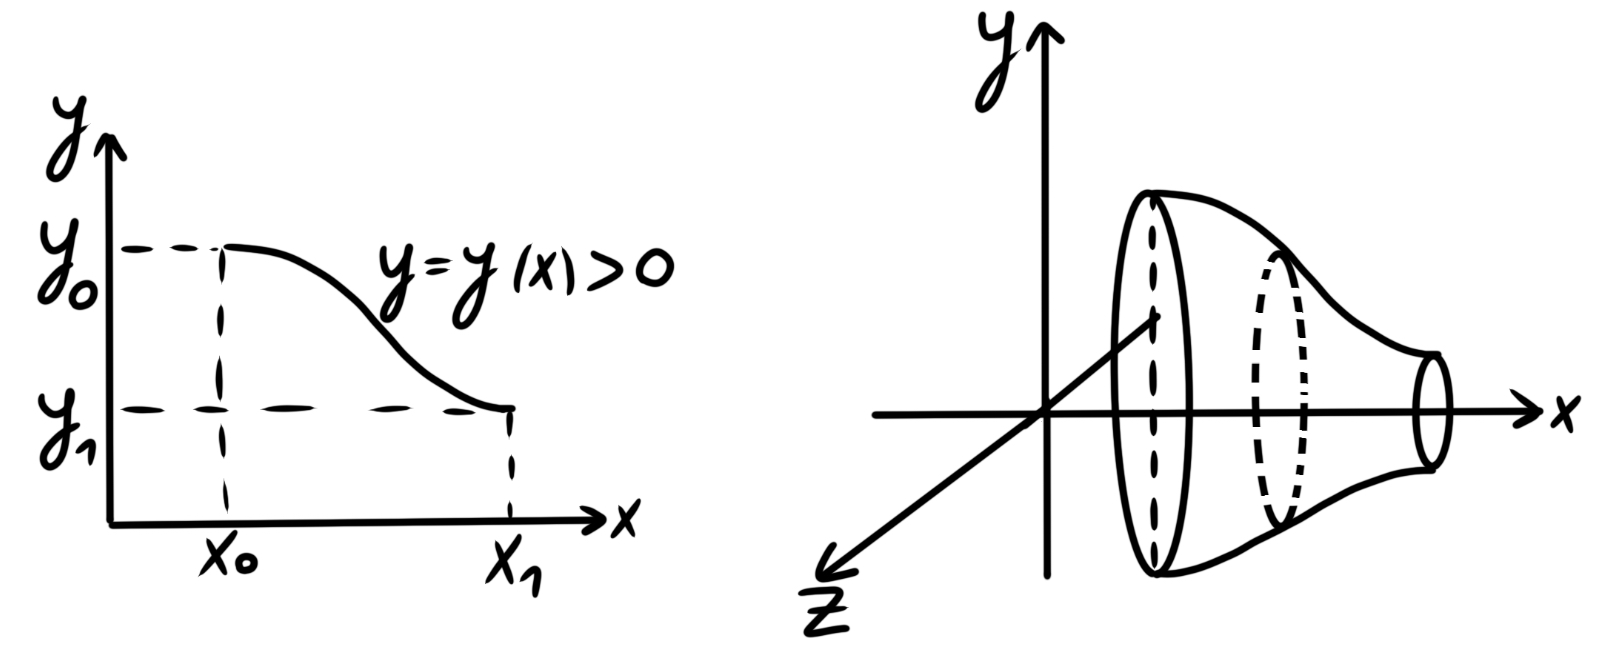
\includegraphics[width=0.8\textwidth]{/Users/vladbelousov/Desktop/Semestr_4-FP-NSU/ДфУ/Лекции_по_дням/image/2.png}
\end{center}

Площадь \( S \to \min  \) 

\begin{center}
    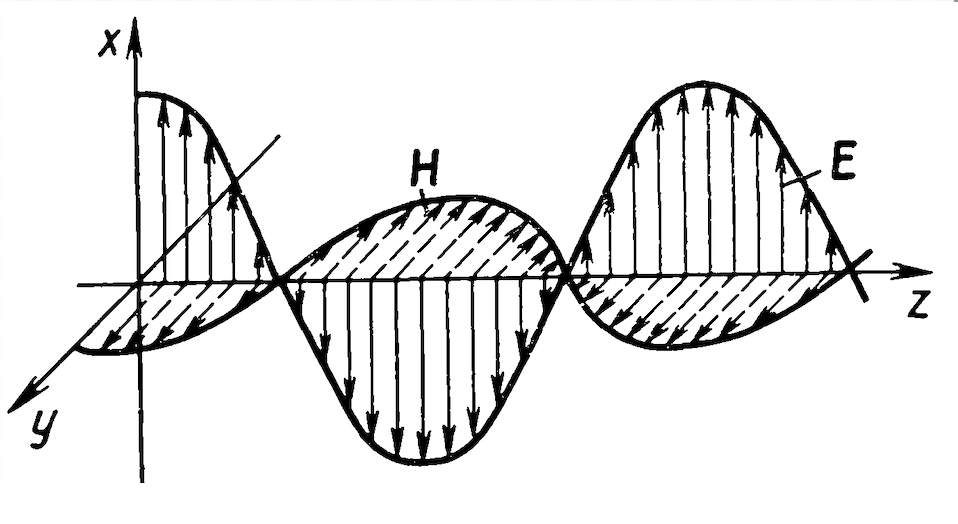
\includegraphics[width=0.5\textwidth]{/Users/vladbelousov/Desktop/Semestr_4-FP-NSU/ДфУ/Лекции_по_дням/image/3.png}
\end{center}

\begin{gather*}
    \Delta \delta= \sqrt{(\Delta x ) ^2 + ( \Delta y) ^2} = \sqrt{1 + \left( \frac{\Delta y}{\Delta x}  \right) ^2} \Delta x \\
    \Delta S = 2 \pi y (x) \Delta \delta \\
    \sum  \Delta S \xrightarrow{\Delta x \to  0}  \int_{x_1}^{x_2} 2 \pi y(x ) \sqrt{1+(y'(x))^2}dx  
\end{gather*}


\begin{flushleft}
    Пример 3 : задача о геодезических на поверхности.
\end{flushleft}

Найти кривую, проходящую через точки А и В, лежащую на поверхности, которая имеет наименьшую длину.

\begin{center}
    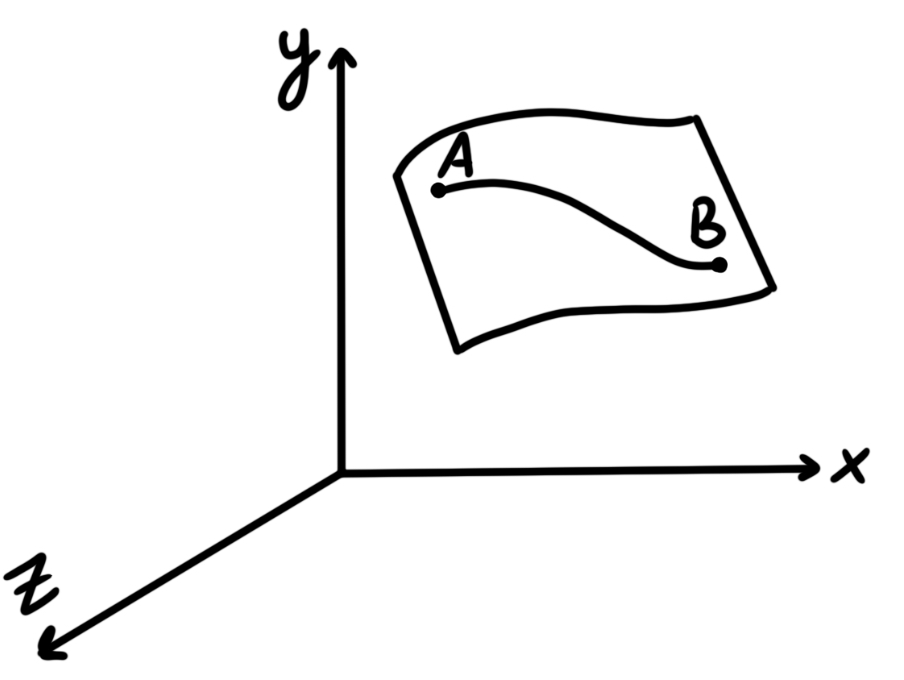
\includegraphics[width=0.4\textwidth]{/Users/vladbelousov/Desktop/Semestr_4-FP-NSU/ДфУ/Лекции_по_дням/image/4.png}
\end{center}
\begin{gather*}
    G(x,y,z)=0 - \text{уравнение поверхности} \\ 
    \text{Пусть уравнение кривой }:
    \begin{cases}
        x=x(t) \\
        y=y(t) \quad \quad t \in  [t_0,t_1] - \text{параметр} \\
        z= z(t)
    \end{cases}\\
    G(x(t),y(t),z(t)) = 0 \leftarrow \text{кривая лежит на поверхности}  \\
    l= \sum  \Delta l = \sum \sqrt{(\Delta x) ^2 + ( \Delta y ) ^2 + ( \Delta z ) ^2}=\sum  \sqrt{\left( \frac{\Delta x}{\Delta t} \right) ^2 + \left( \frac{\Delta y}{\Delta t} \right) ^2 + \left( \frac{\Delta z}{\Delta t} \right) ^2} \Delta t \\
    l \xrightarrow{\Delta t \to  0}    \int_{t_0}^{t_1} \sqrt{(x'(t)) ^2 + ( y'(t)) ^2 + ( z' ( t)) ^2 }dt  
\end{gather*}

\section{Простейшая задача вариационного исчисления}

\[ I[y]= \int_{x_0}^{x_1} F ( x, y(x),y'(x))dx \quad \quad \quad \quad (1)  \] 

\( F : \mathbb{D} \to \mathbb{R}, \mathbb{D} \subset \mathbb{R} ^3   \) непустое открытое множество, \( F \in  C ^2 (\mathbb{D}) \) 

\begin{definition}[допустимая функция]   
    Функция \( y : [x_0,x_1]\to \mathbb{R}  \) называется допустимой, если: 
    
    1) \(\displaystyle  y(x)\in  C([x_0,x_1]) \)
    
    2) \(\displaystyle  y(x) \in  C ^2 ((x_0,x_1)) \)
    
    3) \( \displaystyle \forall x \in  [x_0,x_1 ] , ( x, y(x), y ' (x)) \in  \mathbb{D}  \)
    
    4) \( \displaystyle \int_{x_0 }^{x_1} F(x,y(x),y' (x))dx \)  сходится

\end{definition}



\[ \text{Краевые условия: } y(x_0)=y_0,\text{ }  y(x_1)=y_1 \quad \quad \quad \quad (2) \] 

\begin{definition}
    Допустимая \( \tilde{y}:[x_0,x_1] \to  \mathbb{R}  \) доставляет локальный минимум функционалу (1) при краевых условиях (2),если: 

    1) \( \tilde{y}(x_0)=y_0, \tilde{y}(x_1)= y_1   \) 

    2) \( \exists \varepsilon_0 >0 \text{ }  \forall   \) допустимой функции \( y(x) \), удовлетворяющей (2): \( \sup _{x \in  [x_0,x_1]}|y(x)-\tilde{y}(x) |< \varepsilon_0  \) выполняется: \( I[\tilde{y}] \le I[y] \) 
\end{definition}

\begin{definition}
    Допустимая функция \( \tilde{y} : [x_0,x_1] \to  \mathbb{R} \)  доставляет глобальный минимум функционалу I[y] при краевых условиях (2), если: 

    1) \( \tilde{y} (x_0)=y_0, \text{ } \tilde{y} (x_1) =y_1 \)
    
    2) \( \forall \) допустимой функции \( y(x) \), удовлетворяющей (2), выполняется \( I[\tilde{y} ] \le I [y] \) 
\end{definition}

\section{Необходимые условия локального экстремума}

Аналог \( f'(x) = 0  \) 

Пусть функция \(\tilde{y}   \) доставляет функционалу \( I[y] \) при краевых условиях (2) локальный минимум \( \Rightarrow I[\tilde{y} ] \le I[y]  \), где \( y(x) \) из определенного локального минимума.

Возьмем \( \displaystyle y(x)=\tilde{y} + \varepsilon \eta(x) , \quad \varepsilon \in \left( -\frac{\varepsilon_0}{M}, \frac{\varepsilon_0}{M}   \right), \quad  M= \max _{x \in  [x_0,x_1]} |\eta (x) |  \)

\( \eta (x) \in  C ^2 ([x_0,x_1])  \) - финитная функция. 

\begin{minipage}{0.4\textwidth}
    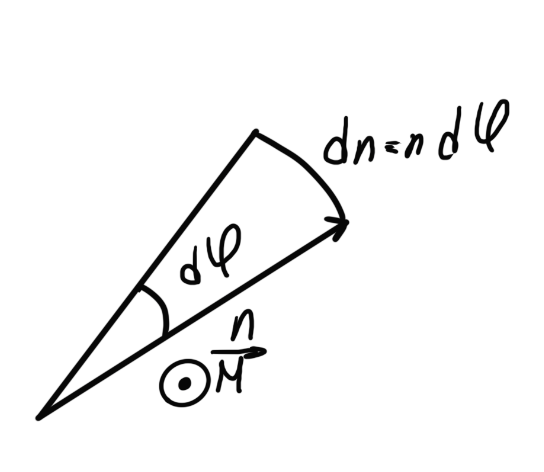
\includegraphics[width=\textwidth]{/Users/vladbelousov/Desktop/Semestr_4-FP-NSU/ДфУ/Лекции_по_дням/image/5.png}
\end{minipage}
\begin{minipage}{1\textwidth}
    \( \quad \quad \quad  \Rightarrow I[\tilde{y} ] \le I[\tilde{y} + \varepsilon \eta ]  \) 
\end{minipage}

Рассмотрим функцию \( g(\varepsilon)= I[\tilde{y}+ \varepsilon \eta  ] \Rightarrow g(0) \le g(\varepsilon) \) 

\begin{minipage}{0.25\textwidth}
    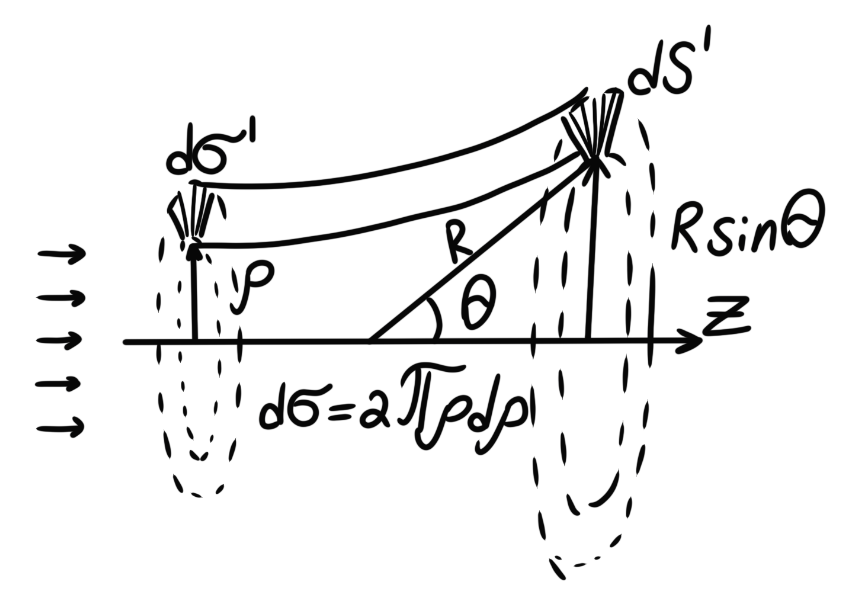
\includegraphics[width=\textwidth]{/Users/vladbelousov/Desktop/Semestr_4-FP-NSU/ДфУ/Лекции_по_дням/image/6.png}
\end{minipage}
\begin{minipage}{1\textwidth}
    \( \quad \varepsilon= 0 - \text{ точка локального минимума для функции } g(\varepsilon) \Rightarrow g'_{\varepsilon}(0)=0     \) 
\end{minipage}

\begin{gather*}
    0 = \frac{d}{d \varepsilon}g (\varepsilon) |_{\varepsilon=0}= \frac{d}{d \varepsilon} \left[ \int_{x_0}^{x_1} F(x,\tilde{y}+ \varepsilon\eta  (x) , \tilde{y}'+\varepsilon\eta ' (x) ) dx \right] \bigg |_{\varepsilon=0} \boxed{=}   \\
    \int_{x_0}^{x_1}= \underbrace{\int_{x_0}^{x_0+\delta} }_{(1)} +   \underbrace{\int_{x_0 +\delta}^{x_1-\delta} }_{(2)}  +\underbrace{\int_{x_1 -\delta}^{x_1} }_{(3)} \quad ; \quad \frac{d}{d \varepsilon} I_1= \frac{d}{d \varepsilon} I_2=0 \\   
\end{gather*}
\begin{theorem}[из математического анализа]
    \( f(x, \varepsilon): [a,b] \times [c,d] \to \mathbb{R}  \) - непрерывна, \( \displaystyle \exists  \frac{df}{d \varepsilon} (x, \varepsilon)   \)  - непрерывна
    \[ \Rightarrow \frac{d}{d \varepsilon} \int_{a}^{b} f(x, \varepsilon)dx= \int_{a }^{b } \frac{d}{d \varepsilon } f(x, \varepsilon)dx     \]  
\end{theorem}  

Вносим производную под знак интеграла: 

\begin{gather*}
    \boxed{=} \int_{x_0 + \delta}^{x_1- \delta}\left[ \frac{\partial F}{\partial y }(\dots) \eta (x )+ \frac{\partial F}{\partial y'} \eta '(x)   \right] dx \bigg |_{\varepsilon=0}=   \int_{x_0 + \delta}^{x_1- \delta}\frac{\partial F}{\partial y }(\dots) \eta (x )dx+ \underbrace{\frac{\partial F}{\partial y'}(x) \eta (x) \bigg |^{x_1- \delta}_{x_0+\delta}    }_{=0}- \\
    -\int_{x_0 + \delta}^{x_1- \delta} \eta (x )\frac{d}{dx } \left[ \frac{\partial F}{\partial y' }(\dots) \right] dx \bigg | _{\varepsilon=0} =\int_{x_0 + \delta}^{x_1- \delta} \left[ \frac{\partial F}{\partial y}(\dots)- \frac{\partial}{\partial x} \frac{\partial F}{\partial y'}(\dots)    \right]\eta(x) dx \bigg |_{\varepsilon=0}  \boxed{=}  \\
    \boxed{=} \int_{x_0 }^{x_1} \eta(x) \left[ \frac{\partial F}{\partial y}(x,y(x),y'(x)) -  \dots \right] dx =0
\end{gather*}

\( \forall   \) финитной функции \( \eta (x)  \)

\begin{lemma}[основаная леммая вариационного исчисления]
    \( f(x) : [x_0,x_1] \to  \mathbb{R} -\) непрерывна и  \( \displaystyle \int_{x_0}^{x_1} f(x)\eta (x)dx=0, \forall   \) финитной \( \eta (x) \). Тогда \( f(x) \equiv 0 \text{ } \forall x \in  [x_0,x_1]   \) 
\end{lemma}

По лемме: \( \displaystyle \frac{\partial F}{\partial y}- \frac{d}{dx} \frac{\partial F}{\partial y '} =0     \) - необходимое условие локального экстремума( \textbf{уравнение Эйлера} )

\begin{definition}[экстремаль]
    Допустимая функция \( y(x) \) называется экстремалью функционала \( I[y] \)  при краевых условиях (2), если: 

    1) \( y(x_0)=y_0, \text{ } y(x_1)=y_1  \) 

    2) \( y(x) \) удовлетворяет условию Эйлера
\end{definition}


%%-------------------------------%%

% Закрытие документа, если файл компилируется отдельно
\ifdefined\mainfile
    % Если это основной файл, не нужно заканчивать документ
\else
    \end{document}
\fi